\chapter{Interviews}
\label{ch:interviews}
This chapter contains the approach and the outcome of the interviews with C-level executives of the \gls{ps}. For the interviews, four executives were invited. The executives were carefully selected to have a balance in the scope of the \gls{ps}.
\begin{table}[H]
	\centering
	\resizebox{\textwidth}{!}{%
		\begin{tabular}{p{.15\textwidth}p{.85\textwidth}}
			\toprule
			\textbf{Interviewee} & \textbf{Role} \\%
			\midrule
			1 & A \acrfull{cio} from the Central Government \\%
			2 & A \acrfull{cto} from the Local Government \\%
			3 & A \acrfull{ceo} from an \acrfull{isv} \\%
			4 & A \acrfull{coo} from a Service Provider \\%
			\bottomrule
		\end{tabular}
	}%
	\caption[Interviewees]{Interviewees}%
	\label{tab:Interviewees}%
\end{table}
The purpose of the interviews was to research the state of \gls{antifragility} and \acrshort{ea} in the \gls{ps}. Since interviews are under a time constraint, it was not possible to talk about every \gls{attribute} separately. Because of this, the research questions were created based on themes. The themes were carefully selected to make sure that there is a possibility that the \glspl{attribute} are mentioned in the conversation. Fore more information on how the themes are connected to the \glspl{attribute} see Appendix~\ref{app:cmapinterviewattributes}. Because the interviews were at C-level, the interviews were not in-depth. It was not possible to talk in-depth about the attributes of \acrshort{ea}. One C-level interviewee became even irritated with a simple question on \acrshort{ea}. Because of this, the interviews are analysed on the schools of thought \parencite{Lapalme2012} of \acrshort{ea}. The attributes are implicitly part of that particular school of thought based on the answers. \cref{tab:interviewquestions} contains the questions that were asked during the interviews. An interview lasted approximately one full hour. The interviews were recorded and automatically transcribed (in Dutch). The interviewee gave consent for the recording and transcription. It is not possible to make the recordings and the transcriptions anonymous to be part of the publicly available data set. In place of sharing the recordings and the transcriptions, the thesis has summaries of the interviews attached. See Appendix~\ref{app:interviewsummaries} for these summaries. The Antwerp Management School can request the recordings and transcriptions only for (re)accreditations and visitations to enable the Antwerp Management School to comply with statutory obligations.
\begin{table}[H]
	\centering
	\resizebox{\textwidth}{!}{%
		\begin{tabular}{@{}p{0.1\textwidth}p{0.75\textwidth}p{0.15\textwidth}@{}}
			\toprule
			\textbf{Number} & \textbf{Question} & \textbf{Concept} \\ \midrule %
			1a. & How is your organisation applying \acrshort{ea}? & \acrshort{ea} \\%
			1b. & Who is accountable for \acrshort{ea} in your organisation? & \acrshort{ea} \\%
			1c. & How is \acrshort{ea} enabling your organisation to quickly adapt to changes (external influences)? & \acrshort{ea} \\%
			2a. & Does the operational model of the\gls{ps} \gls{foster} \gls{agility}? & \Gls{antifragile} \\%
			2b. & How is the \acrshort{ea} of your organisation contributing to \gls{foster} \gls{agility} in the \gls{ps}? & \acrshort{ea} \\%
			3a. & How does the public sector deal with \gls{uncertainty}? & \Gls{antifragile} \\%
			3b. & How is the \acrshort{ea} of your organisation contributing to dealing with \gls{uncertainty} in the \gls{ps}?
			& \acrshort{ea} \\%
			4a. & How is the public sector dealing with unexpected events? & \Gls{antifragile} \\%
			4b. & How is \acrshort{ea} of your organisation contributing to dealing with unexpected events in the \gls{ps}? & \acrshort{ea} \\%
			5a. & Could you describe the risk appetite of the \gls{ps}? & \Gls{antifragile} \\%
			5b. & How does the \acrshort{ea} of your organisation match the risk appetite of the \gls{ps}?
			& \acrshort{ea} \\%
			6a. & How is \gls{diversity} and \gls{optionality} used in the \gls{ps}? & \Gls{antifragile} \\%
			6b. & How does \acrshort{ea} of your organisation support \gls{diversity} and \gls{optionality} in the \gls{ps}? & \acrshort{ea} \\%																								
			Closing & Did you miss an important subject or do you want to add something else? & non-specific \\%
			\bottomrule
		\end{tabular}
	}%
		\caption[Interview questions]{Interview questions}
		\label{tab:interviewquestions}
\end{table}
\section{Interview results}
After the interviews \acrfull{qda} took place. For \acrshort{qda}, the transcriptions of the interviews were used and coded with labels. A label was created for every positive and negative version of an \gls{attribute} (\gls{antifragile} and no \gls{antifragile}). While doing the \acrshort{qda} possible new \glspl{attribute} are discovered. Labels are also created for these new attributes. After coding analysis was started. The data set of this analysis is available as a structured Microsoft Excel workbook with multiple worksheets. This file is available in the GitHub repository of this research\footnote{\url{https://github.com/JRBliekendaal/master-thesis/blob/main/datasets/interviews/raw_interview_data_and_charts.xlsx}}. The interview results are discussed through a description supported by a set of graphs. One graph is the number of times an \gls{attribute} was mentioned, the frequency, and the other graph is the percentage of the interviews in which this was mentioned, \% of Cases. The discussion will take place based on the earlier defined categories \gls{attenuatevariety}, \gls{amplifyvariety}, Learning organisation and the \acrlong{ea} schools of thought. The charts have to be read as if a \gls{attribute} scores positive the \gls{attribute} is present. When the an \gls{attribute} scores negatively the \gls{attribute} is not present or is missed. This mean, based on the used data set, that the \gls{attribute} could be a success factor.
\subsection{Interview results on Attenuate variety}
\label{sub:interviewresultsattenuate}
\begin{figure}[H]
	\centering
	\begin{subfigure}[H]{0.5\textwidth}
		\centering
		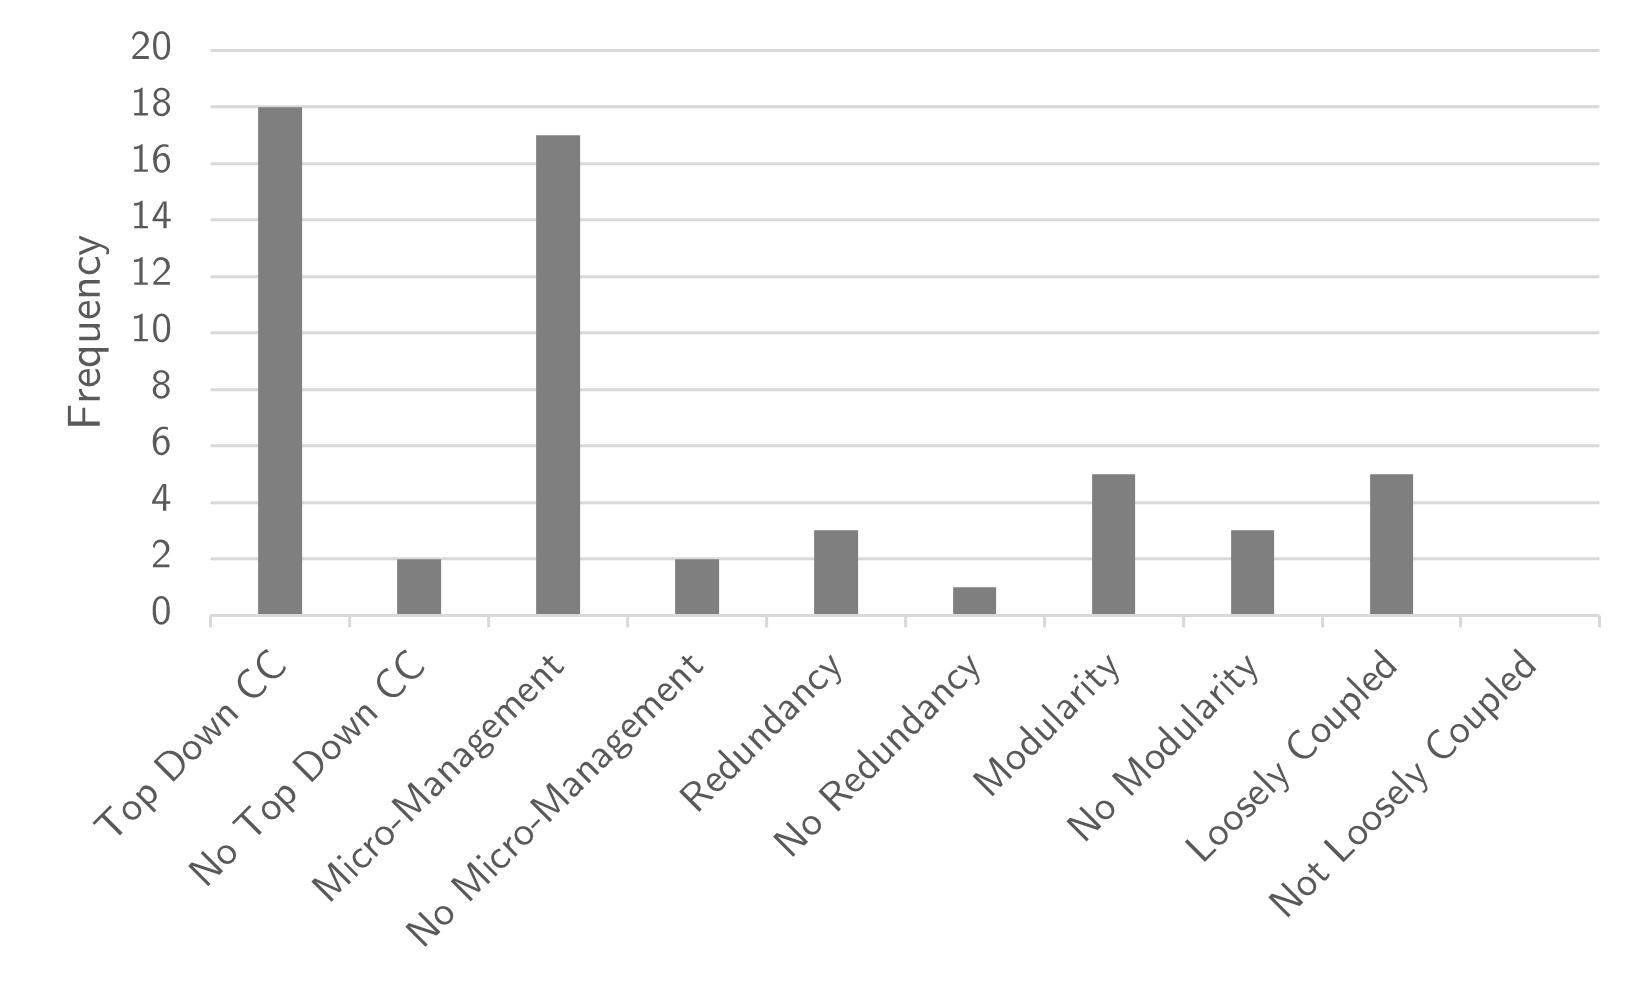
\includegraphics[width=0.95\linewidth]{images/attenuate_frequency}
		\caption{Attenuate variety Frequency}
		\label{fig:attenuatefrequency}
	\end{subfigure}%
	\begin{subfigure}[H]{0.5\textwidth}
		\centering
		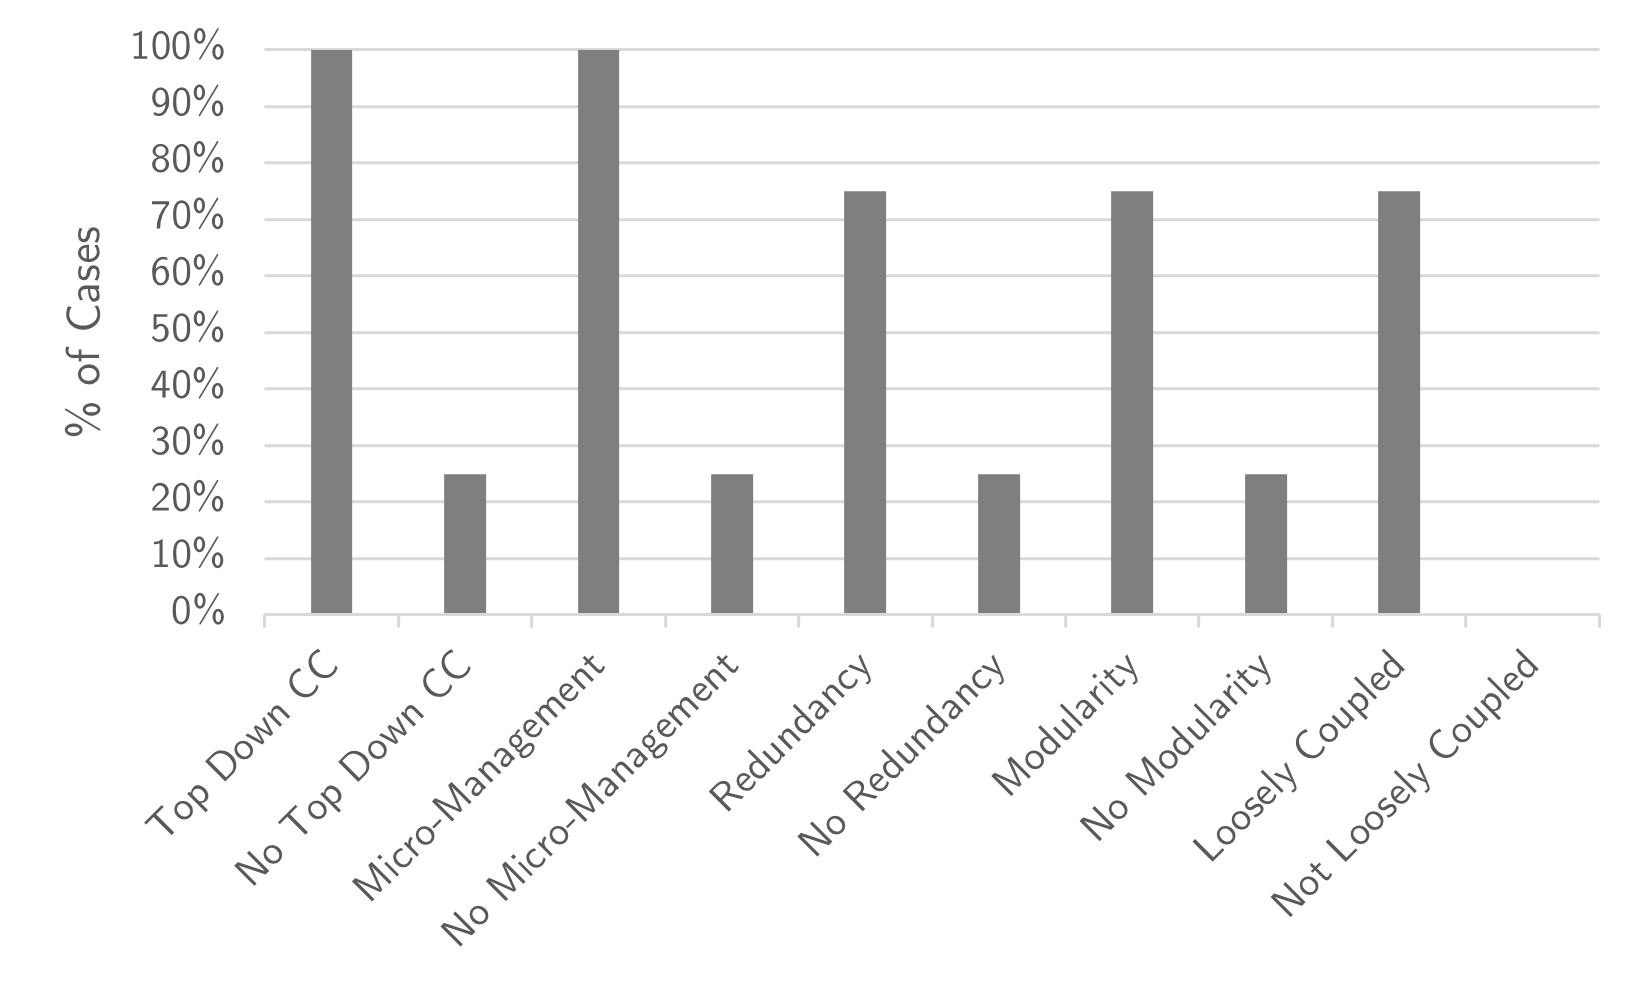
\includegraphics[width=0.95\linewidth]{images/attenuate_cases}
		\caption{Attenuate variety \% of Cases}
		\label{fig:attenuatecases}
	\end{subfigure}
	\caption{Interview results Attenuate variety}
	\label{fig:interviewattenuatevariety}
\end{figure}
Why \textit{\gls{topdowncc}} and \textit{\gls{micromanagement}} scored highly is because the governments in the \gls{ps} have a severe risk-avoiding attitude. Everything must be predefined and planned. There must be accountability for how public money is spent. All missteps are magnified. There is a quick result in crises, but with possible consequences later on because of \acrfull{bit} audits or \glspl{parliamentaryinquiry}. The reflex on \gls{uncertainty} of the \gls{ps} is that the \gls{ps} gets very insecure from \gls{uncertainty}. The \gls{ps} does not know how to deal with \gls{uncertainty}. The common reflex is to push the \gls{uncertainty} back to certainty, so it is under control again. E.g. a missing law with the introduction of electric steps. It is not a bike, not a motorcycle or a car. The electric step did not fit into the current laws and regulations. The result was that the policymakers did not approve it and did not even tolerate it until law-making finished. \Gls{modularity} and \gls{looselycoupled} both scored a bit because the \gls{ps} consists out of a lot of subsystems. Every subsystem has a clear goal and a reason to exist. Communication between subsystems are going through standardised interfaces and are predictable.
\subsection{Interview results on Amplified variety}
\label{sub:interviewresultsaplified}
\begin{figure}[H]
	\centering
	\begin{subfigure}[H]{0.5\textwidth}
		\centering
		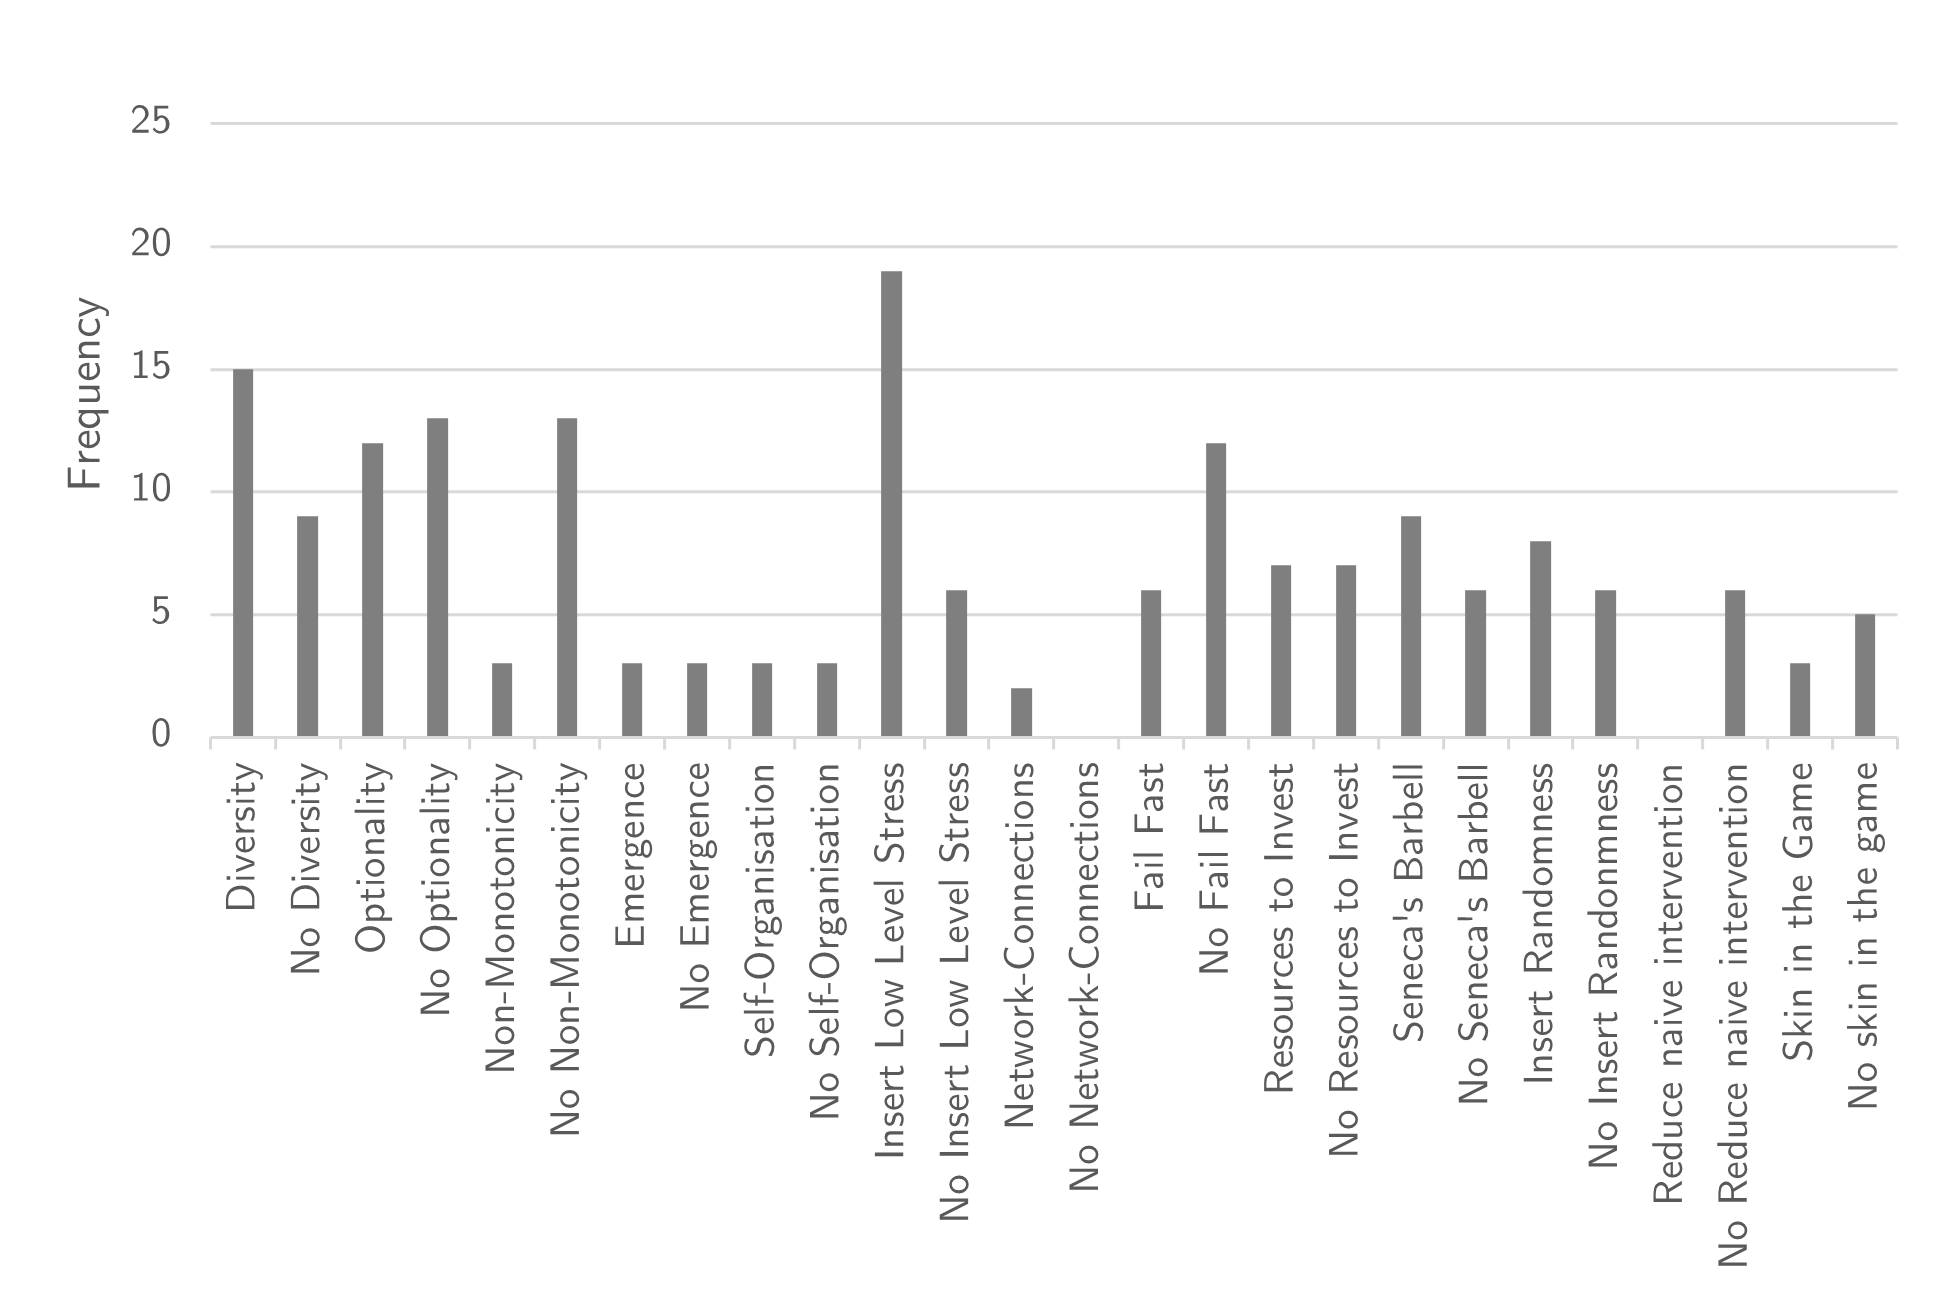
\includegraphics[width=0.95\linewidth]{images/amplified_frequency}
		\caption{Amplified variety Frequency}
		\label{fig:amplifiedfrequency}
	\end{subfigure}%
	\begin{subfigure}[H]{0.5\textwidth}
		\centering
		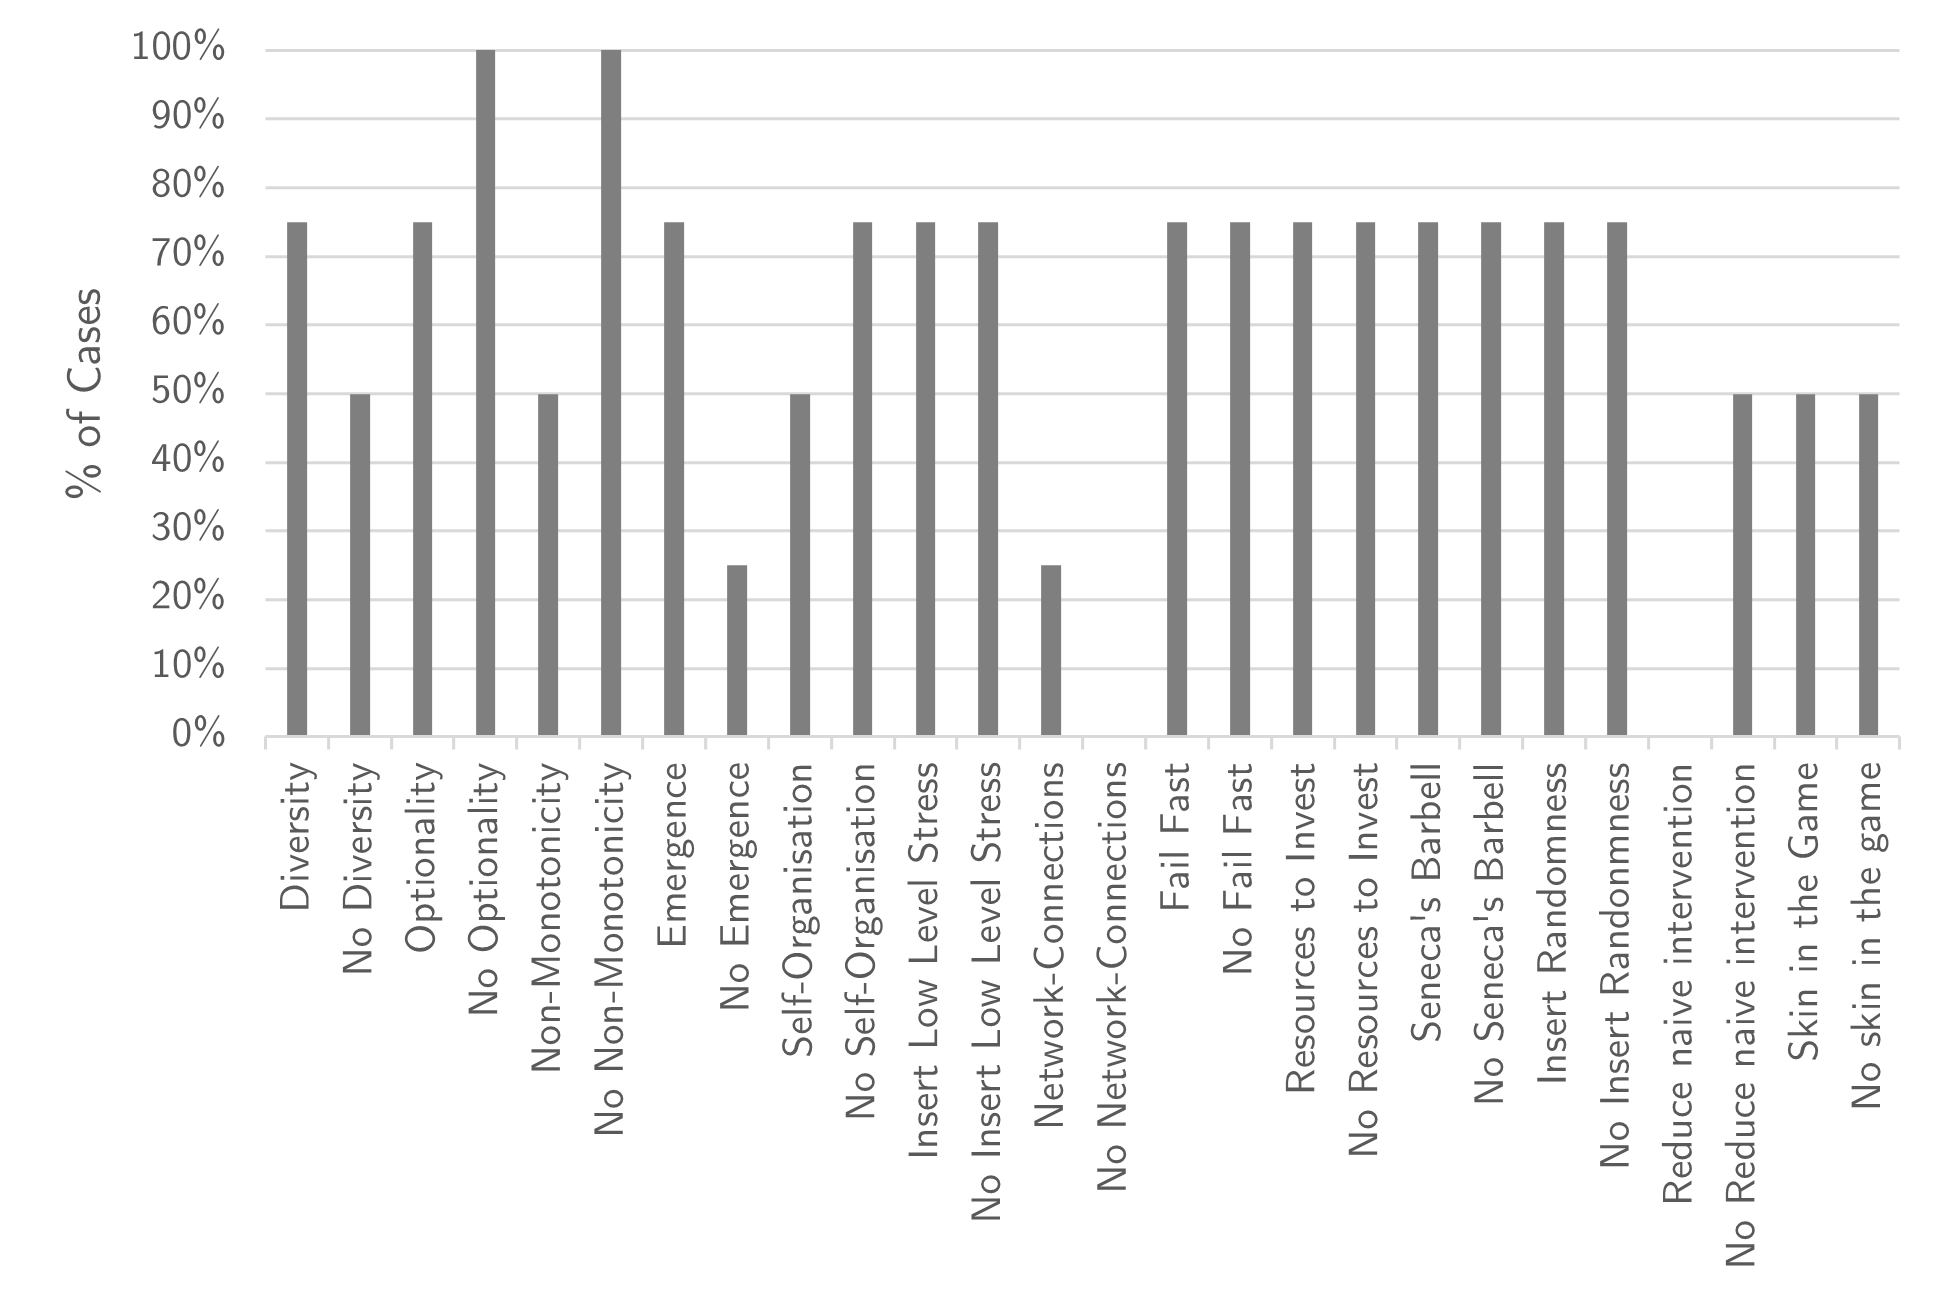
\includegraphics[width=0.95\linewidth]{images/amplified_cases}
		\caption{Amplified variety \% of Cases}
		\label{fig:amplifiedcases}
	\end{subfigure}
	\caption{Interview results Amplified variety}
	\label{fig:interviewamplifiedvariety}
\end{figure}

No optionality and no-monotonicity


One interviewee stated that the \gls{ps} should be in a permanent crisis situation to get things done.

The end goal is not very clear with \gls{agile} working. It is unclear how the public money is spent on precisely what. 



There is no risk appetite. Everything must be known and explainable in advance. If it is found that the procedures are not used, it can result in political consequences later on. Afterwards, positive lessons learned are not used to make adjustments within the public sector. Experimentation is (almost) not possible.

\subsection{Interview results on Learning organisation}
\label{sub:interviewresultslearning}
\begin{figure}[H]
	\centering
	\begin{subfigure}[H]{0.5\textwidth}
		\centering
		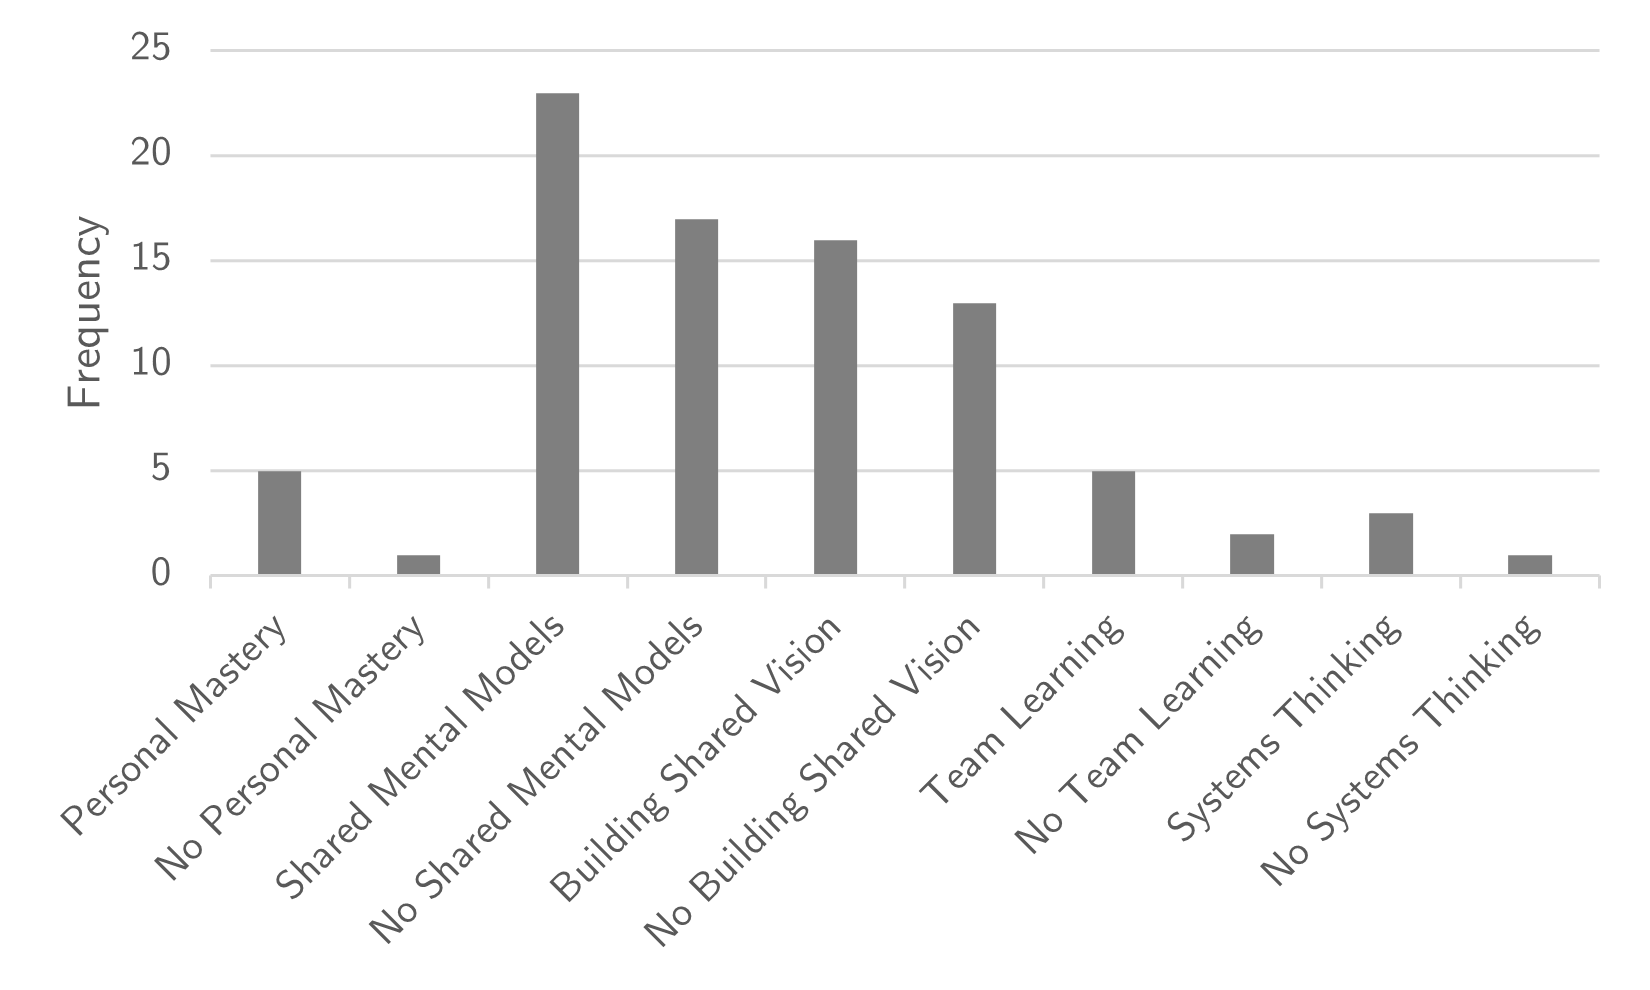
\includegraphics[width=0.95\linewidth]{images/learningorganisation_frequency}
		\caption{Learning organisation Frequency}
		\label{fig:learningfrequency}
	\end{subfigure}%
	\begin{subfigure}[H]{0.5\textwidth}
		\centering
		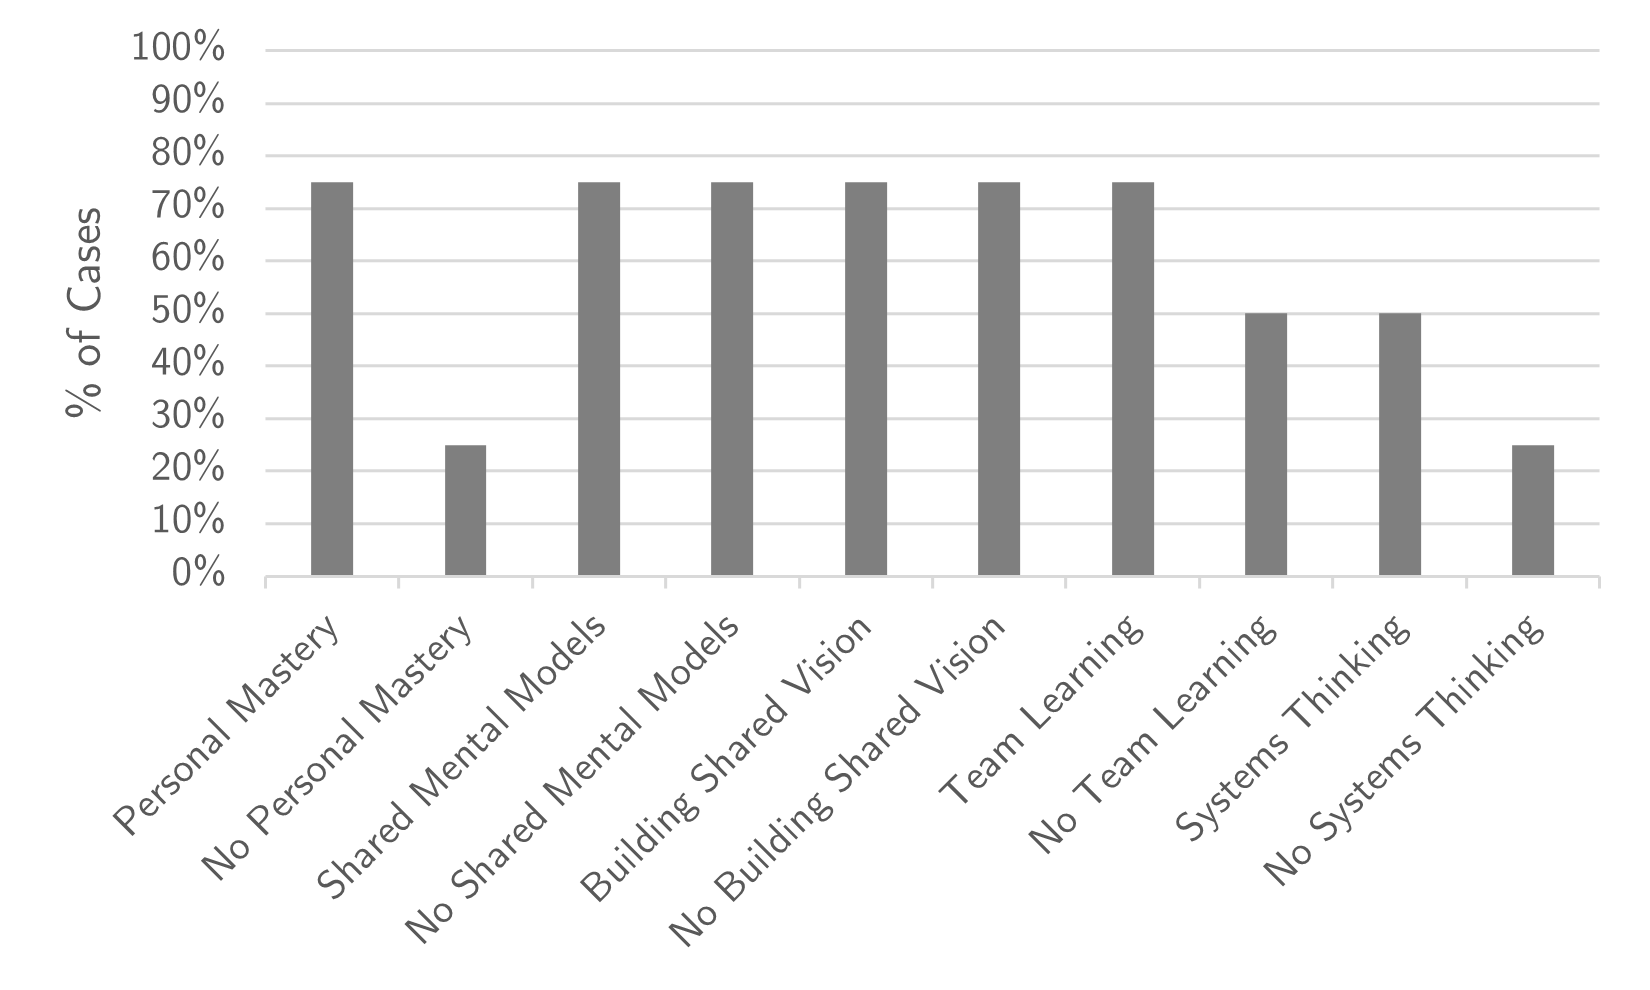
\includegraphics[width=0.95\linewidth]{images/learningorganisation_cases}
		\caption{Learning organisation \% of Cases}
		\label{fig:learningcases}
	\end{subfigure}
	\caption{Interview results Learning organisation}
	\label{fig:interviewlearningorganisation}
\end{figure}

\subsection{Interview results on Enterprise Architecture schools of thought}
\label{sub:interviewresultseaschools}
\begin{figure}[H]
	\centering
	\begin{subfigure}[H]{0.5\textwidth}
		\centering
		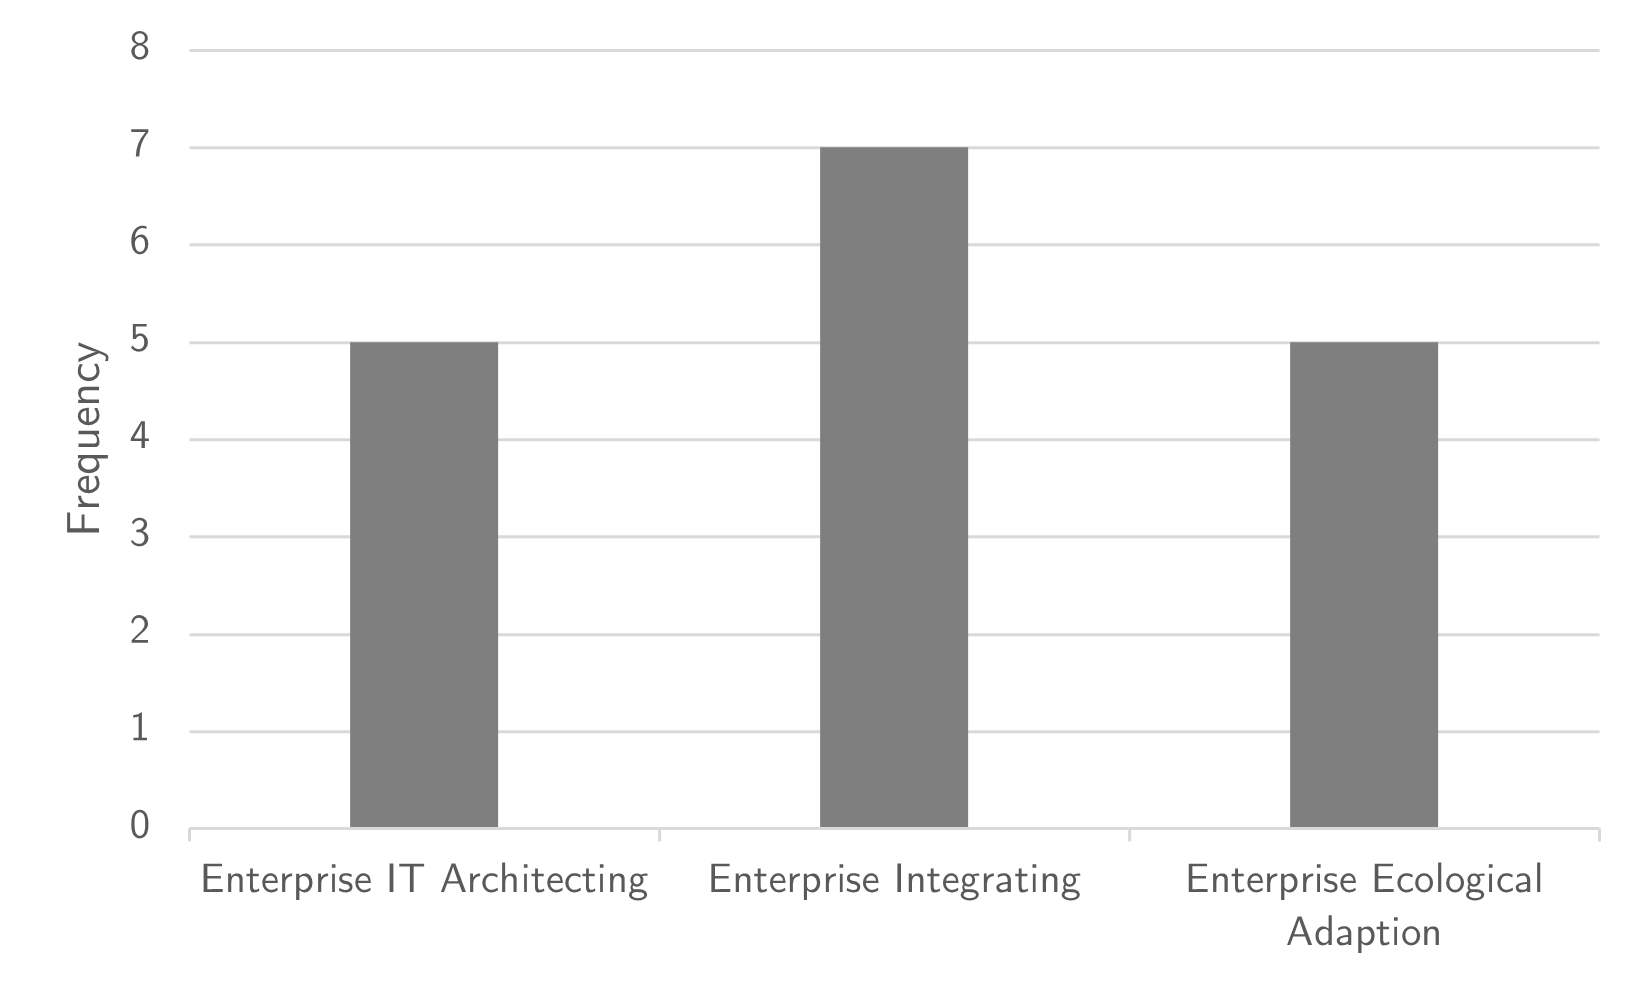
\includegraphics[width=0.95\linewidth]{images/easchools_frequency}
		\caption{Enterprise Architecture Schools of thought Frequency}
		\label{fig:easchoolsfrequency}
	\end{subfigure}%
	\begin{subfigure}[H]{0.5\textwidth}
		\centering
		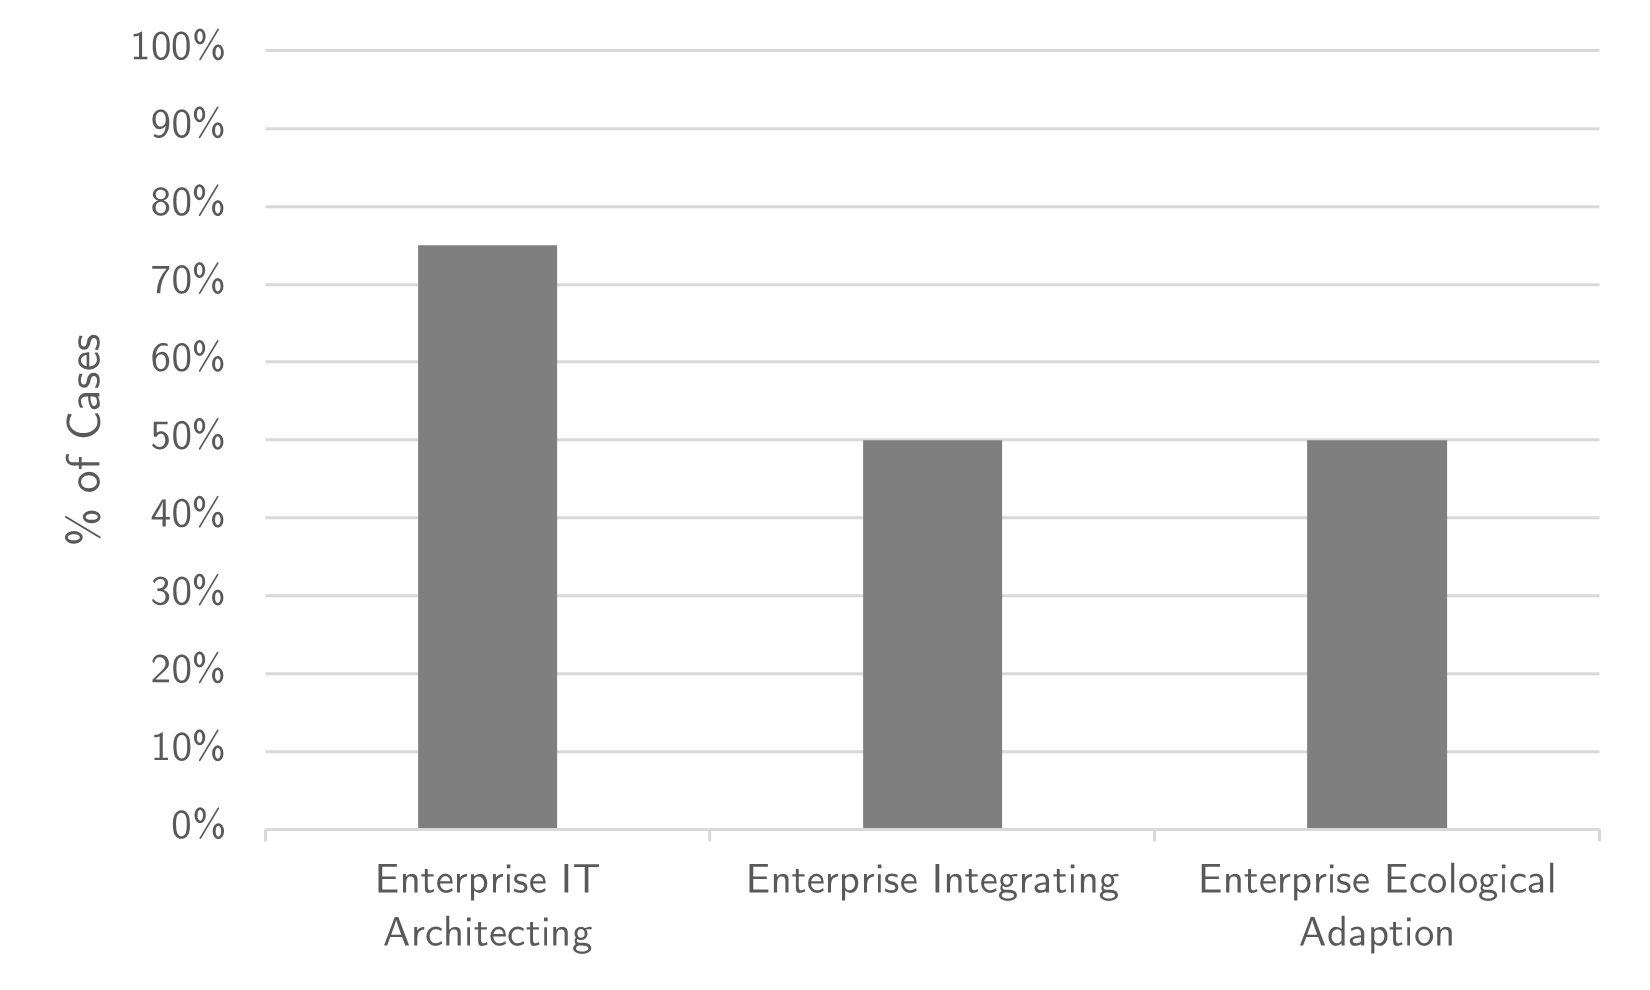
\includegraphics[width=0.95\linewidth]{images/easchools_cases}
		\caption{Enterprise Architecture Schools of thought \% of Cases}
		\label{fig:easchoolscases}
	\end{subfigure}
	\caption{Interview results Enterprise Architecture schools of thought}
	\label{fig:easchoolsantifragile}
\end{figure}



What we have to do in the public sector depends on the political decision making within the period of governing (four years until new elections). \acrshort{ea} is at the end of the chain of administrative decision-making.

\subsection{Interview results on possible new attributes}
\begin{figure}[H]
	\centering
	\begin{subfigure}[H]{0.5\textwidth}
		\centering
		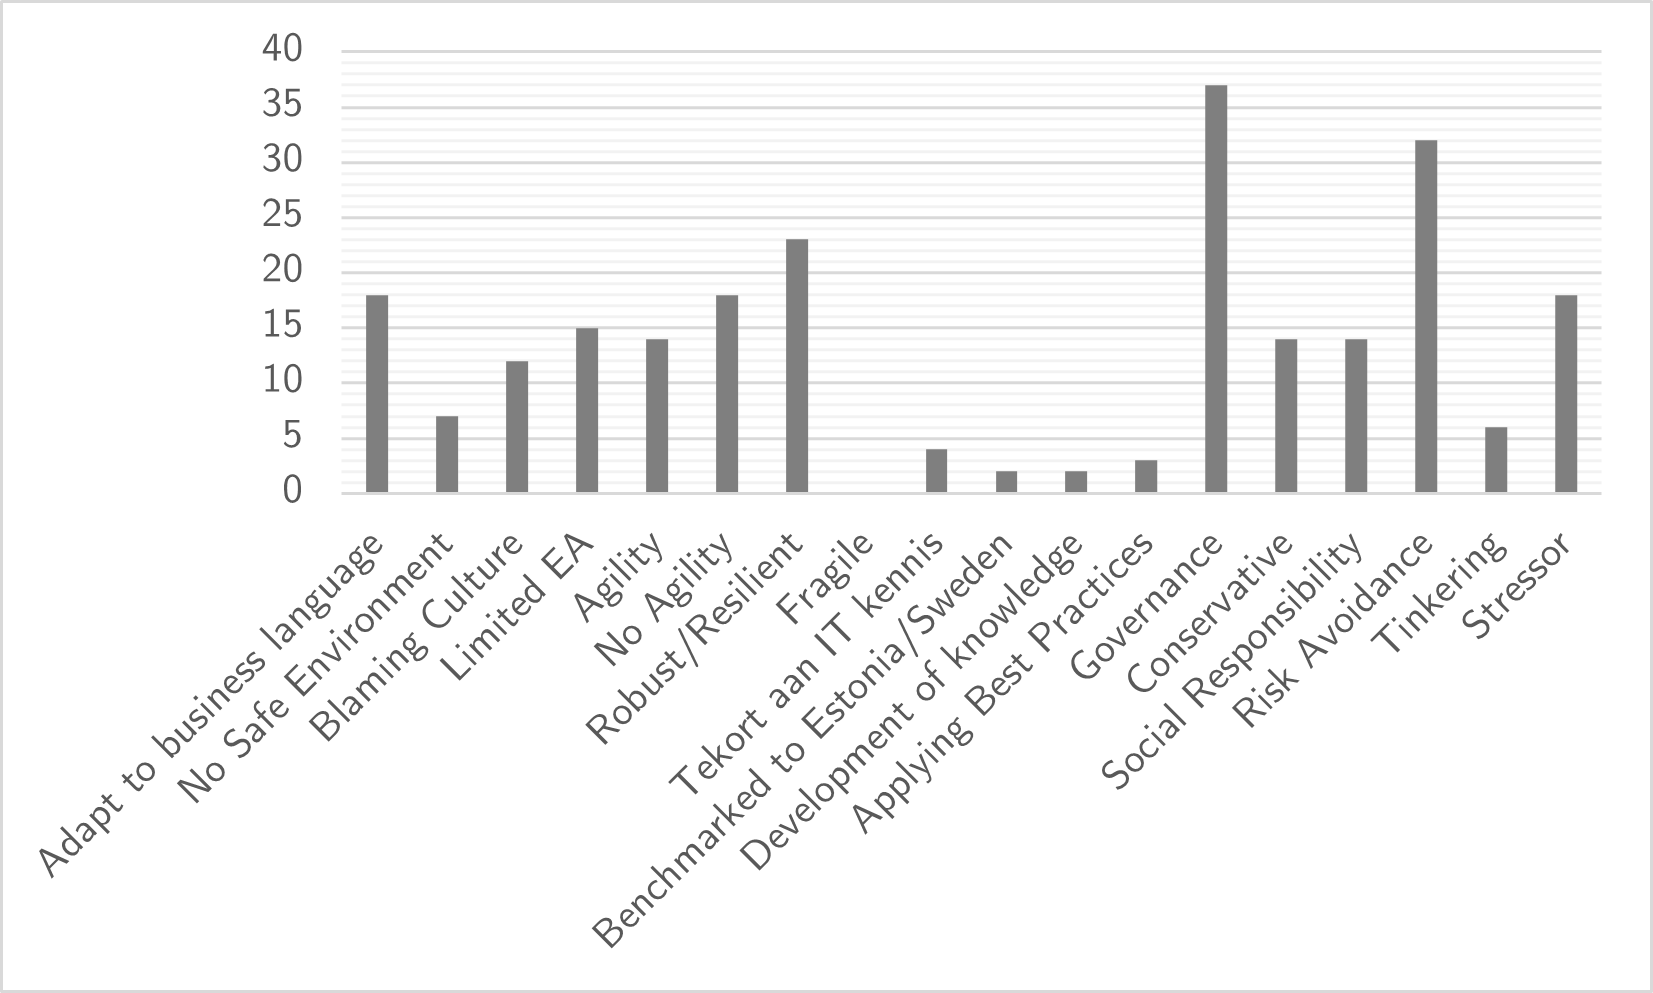
\includegraphics[width=0.95\linewidth]{images/findings_frequency}
		\caption{Findings Frequency}
		\label{fig:findingsfrequency}
	\end{subfigure}%
	\begin{subfigure}[H]{0.5\textwidth}
		\centering
		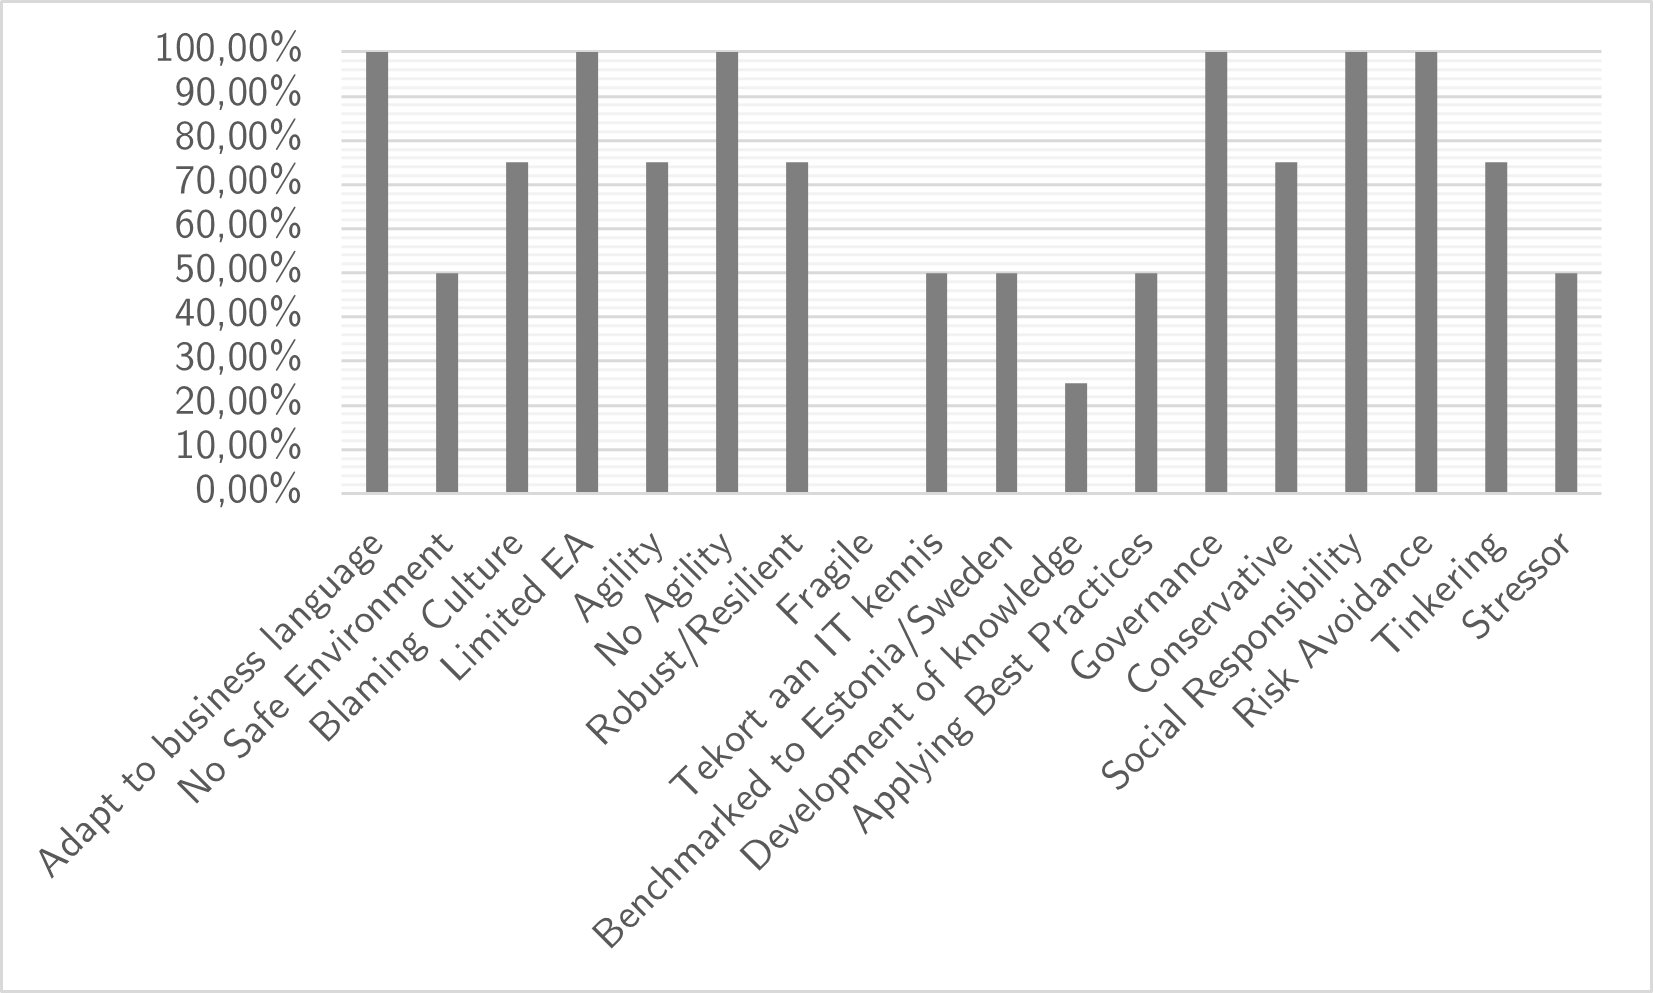
\includegraphics[width=0.95\linewidth]{images/findings_cases}
		\caption{Findings \% of Cases}
		\label{fig:findingscases}
	\end{subfigure}
	\caption{Interview results Findings}
	\label{fig:interviewresultsfindings}
\end{figure}

\section{Qualitative Data Analysis}
\label{sec:dataprep}

\subsection{Merging similar attributes}
\label{sub:merginglabels}
\begin{table}[H]
	\centering
	\resizebox{\textwidth}{!}{%
		\begin{tabular}{p{.05\textwidth}p{.5\textwidth}p{.45\textwidth}}
			\toprule %
			\textbf{Step} & \textbf{Description} & \textbf{Rationale} \\%
			\midrule %
			1	  & Create, positive and negative main categories of Engineering, Systems, CAS, \gls{antifragile}, and Learning organisation. & Need extra categories for merging overarching subjects. \\%
			2     & Merge \gls{agility} into CAS & How \gls{agility} is interpreted is the same as CAS \\%
			3     & Merge tinkering into Learning Organisation & How tinkering is interpreted it is the same as Learning Organisation. \\%
			4     & Merge \gls{robust} and \gls{resilient} into Engineering Resilience & How \gls{robust} and \gls{resilient} is interpreted by interviewees is the same as Engineering Resilience. \\%
			5     & Merge Governance into Engineering Resilience & How Governance is interpreted is the same as \gls{topdowncc} and \gls{micromanagement}. \\%
			6     & Merge Shortage on IT Knowledge into no \gls{resourcestoinvest} & Shortage on IT Knowledge can be interpreted as a resource that is not there \\%
			7     & Merge Applying Best practices into \gls{nonmonotonicity} & Applying Best practices is learning from the past. \\%
			8     & Merge Development of Knowledge into Learning Organisation & Development of Knowledge within an organisation can be seen as the learning capability of an organisation. \\%
			9     & Merge Blaming Culture into No Safe Environment & No Safe Environment is a result of a Blaming Culture. \\%
			10    & Merge Limited \acrshort{ea} into \gls{enterpriseitarchitecting} & Limited \acrshort{ea} is interpreted as the school of thought \gls{enterpriseitarchitecting} \\%
			11    & Merge conservative into Risk Avoidance & Risk Avoidance is a result of conservative \\%
			12	  & Ignored Social Responsibility and Risk Avoidance as \glspl{attribute} as possible success factors & Social Responsibility and Risk Avoidance are attributes of the \gls{ps} and are less relevant as an attribute for \gls{antifragile} and \acrshort{ea}. \\%
			\bottomrule %
		\end{tabular}%
	}%
	\caption{Data preparation - Merging similar labels}
	\label{tab:prepmergingsimilarlabels}%
\end{table}%

\subsection{Normalise frequency of attributes}
\label{sub:normalisefrequency}
To remove (emotional) bias of interviewees the frequency is normalised by only counting the occurrence of an attribute once per question per interview.
\begin{table}[H]
	\centering
	\resizebox{\textwidth}{!}{%
		\begin{tabular}{p{.05\textwidth}p{.5\textwidth}p{.45\textwidth}}
			\toprule %
			\textbf{Step} & \textbf{Description} & \textbf{Rationale} \\%
			\midrule %
			1		&	Count the presence of an \gls{attribute} only once per question per interview. & Removing (emotional) bias. With seven main questions the score of an \gls{attribute} can have a maximum of seven per interview. With four conducted interviews the maximum score of an \gls{attribute} is twenty-eight. \\%
			\bottomrule %
		\end{tabular}%
	}%
	\caption[Data preparation - Normalise frequency of attributes]{Data preparation - Normalise frequency of attributes}
	\label{tab:normalisefrequency}%
\end{table}%

\subsection{Normalise score of attributes}
\label{sub:normalisescore}

\begin{table}[H]
	\centering
	\resizebox{\textwidth}{!}{%
		\begin{tabular}{p{.05\textwidth}p{.5\textwidth}p{.45\textwidth}}
			\toprule %
			\textbf{Step} & \textbf{Description} & \textbf{Rationale} \\%
			\midrule %
			1		&	Add for every lonely negative a 0 positive & Looking for \glspl{attribute} that can be a success factor after normalisation. \\%
			2		&	\Gls{attribute} score is Positive value - Negative value & Bringing the values back to the found \glspl{attribute}. \\%
			3		&	Split up between literature found, \acrshort{ea} and new findings & Categorise. For the literature found there are 2 corners of the triangle. \acrshort{ea} is a different subject than antifragile. The newly found do not have a data point in the literature study of the triangulation. \\%
			\bottomrule %
		\end{tabular}%
	}%
	\caption[Data preparation - Normalise score of attributes]{Data preparation - Normalise score of attributes}
	\label{tab:prepnormalise}%
\end{table}%

\subsection{Filter attributes on threshold 75\% of Cases}
\label{sub:filteronthresholdcases}
\begin{table}[H]
	\centering
	\resizebox{\textwidth}{!}{%
	\begin{tabular}{p{.05\textwidth}p{.5\textwidth}p{.45\textwidth}}
		\toprule %
		\textbf{Step} & \textbf{Description} & \textbf{Rationale} \\%
		\midrule %
		1     & Select labels where \% case is 75\% or more & When three interviewees mentioned the attribute it could be a label of significance (Triangulation) \\%
		\bottomrule
	\end{tabular}%
	}%
	\caption{Data preparation - Filter attributes on threshold 75\% of Cases}
	\label{tab:prepselectcases}%
\end{table}%

\section{Results of Qualitative Data Analysis}

\subsection{Results of QDA Attenuate and Amplified variety}
\label{sub:resultsqdavariety}
\begin{figure}[H]
	\centering
	\begin{subfigure}[H]{0.475\textwidth}
		\centering
		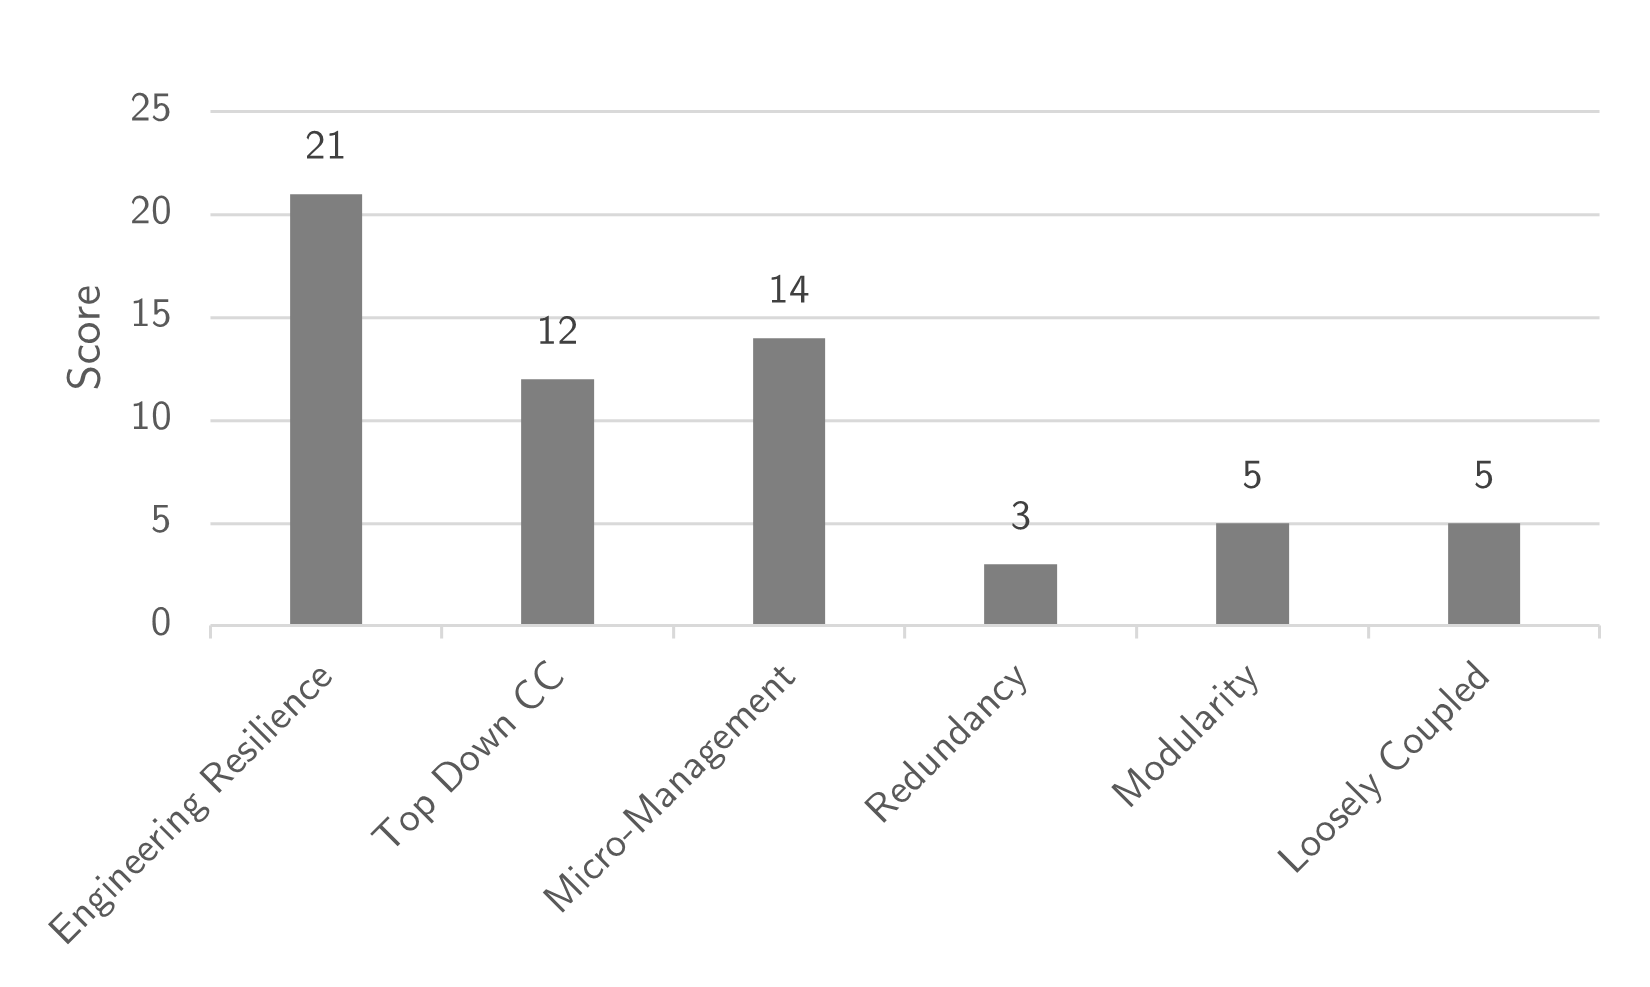
\includegraphics[width=\textwidth]{images/qdaattenuate}
		\caption{QDA Attenuate variety}
		\label{fig:qdaattenuate}
	\end{subfigure}%
\hfill
	\begin{subfigure}[H]{0.475\textwidth}
		\centering
		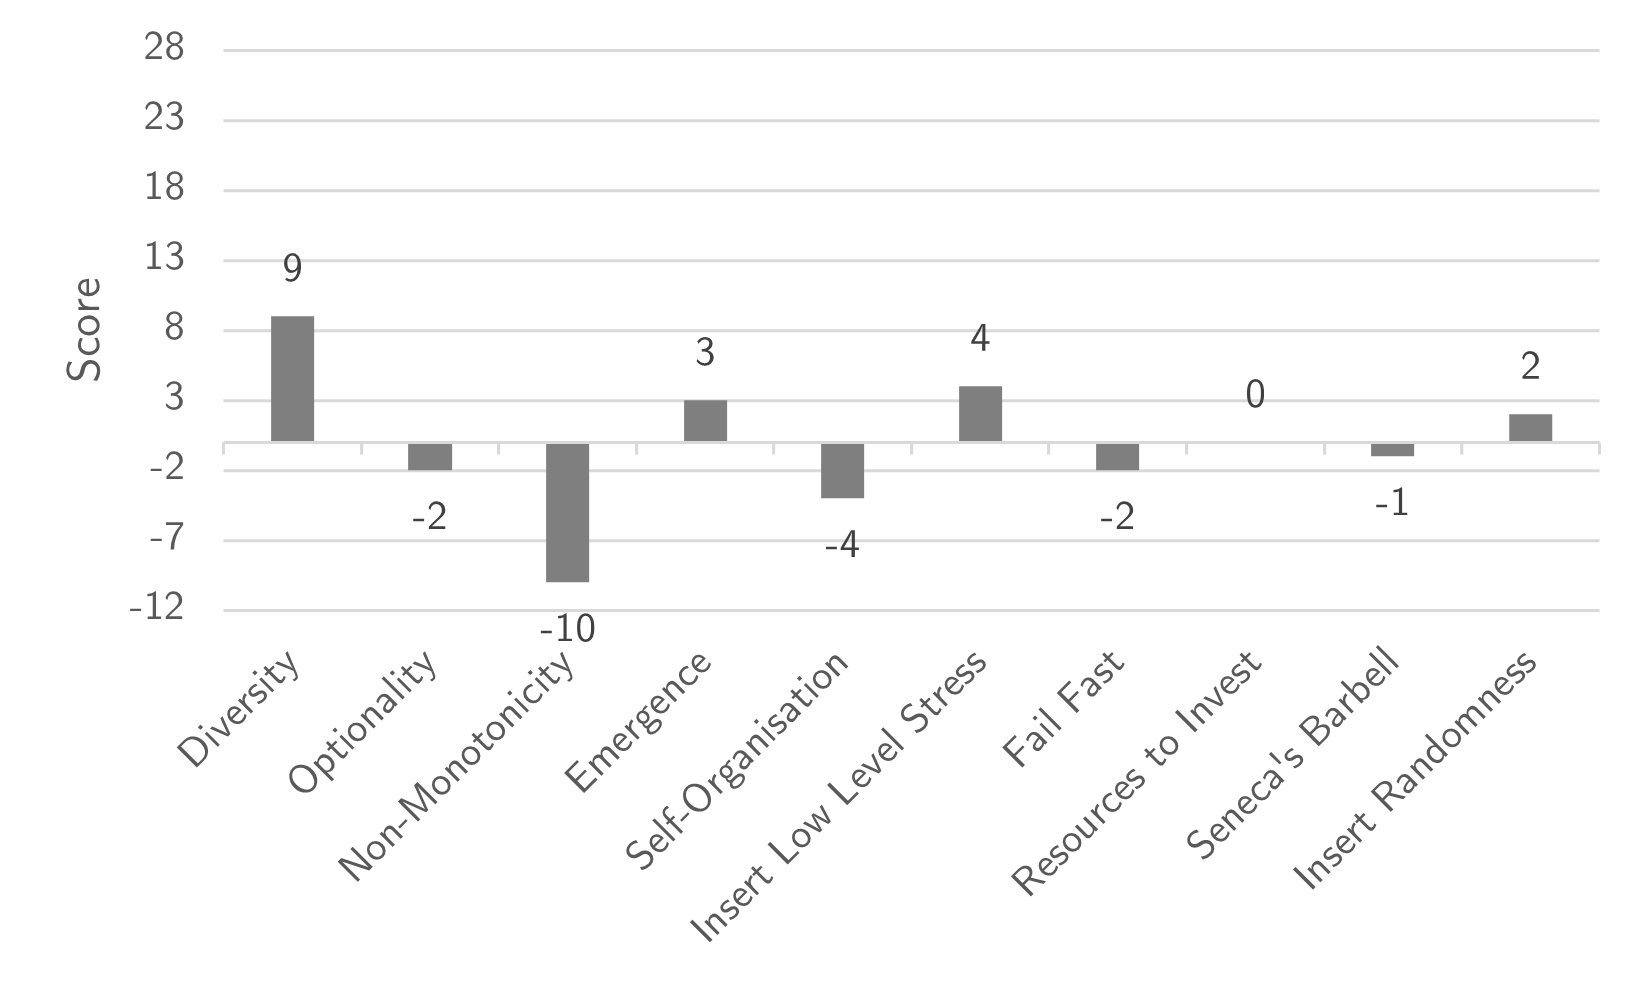
\includegraphics[width=\textwidth]{images/qdaamplify}
		\caption{QDA Amplified variety}
		\label{fig:qdaamplified}
	\end{subfigure}
	\caption{Results of QDA Attenuate and Amplified variety}
	\label{fig:resultsofqdavariety}
\end{figure}

\subsection{Results of QDA Learning organisation and EA school of thought}
\label{sub:resultsqdalearningandea}
\begin{figure}[H]
	\centering
	\begin{subfigure}[H]{0.475\textwidth}
		\centering
		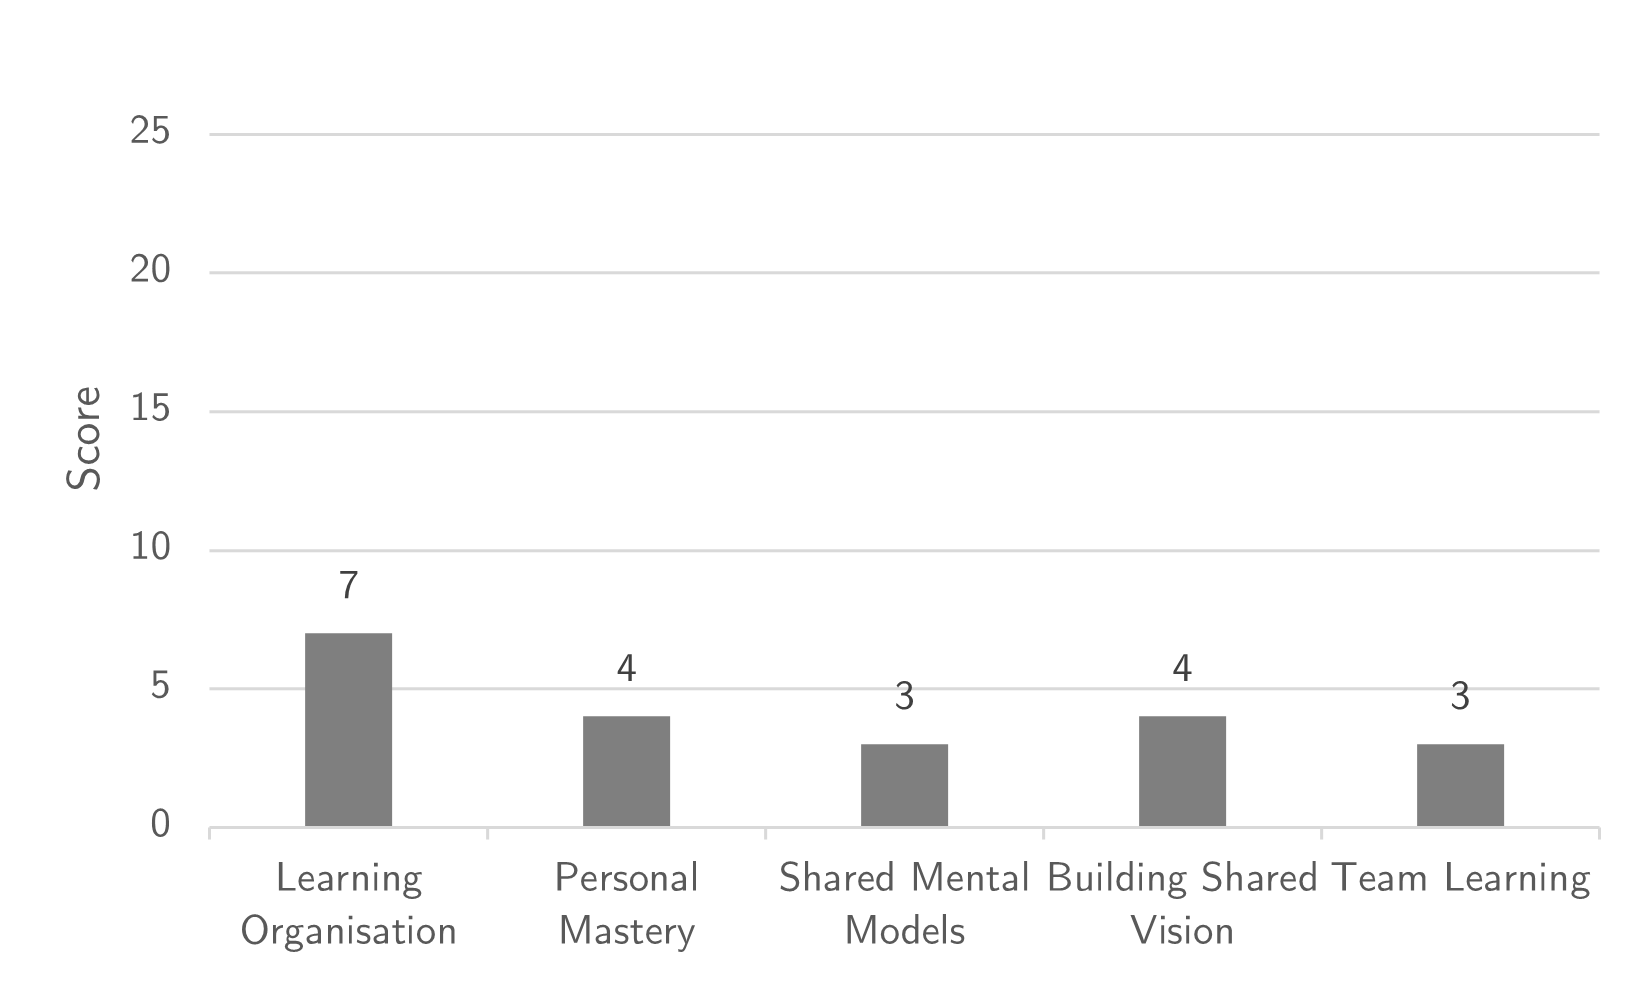
\includegraphics[width=\textwidth]{images/qdalearningorganisation}
		\caption{QDA Learning organisation}
		\label{fig:qdalearning}
	\end{subfigure}%
\hfill
	\begin{subfigure}[H]{0.475\textwidth}
		\centering
		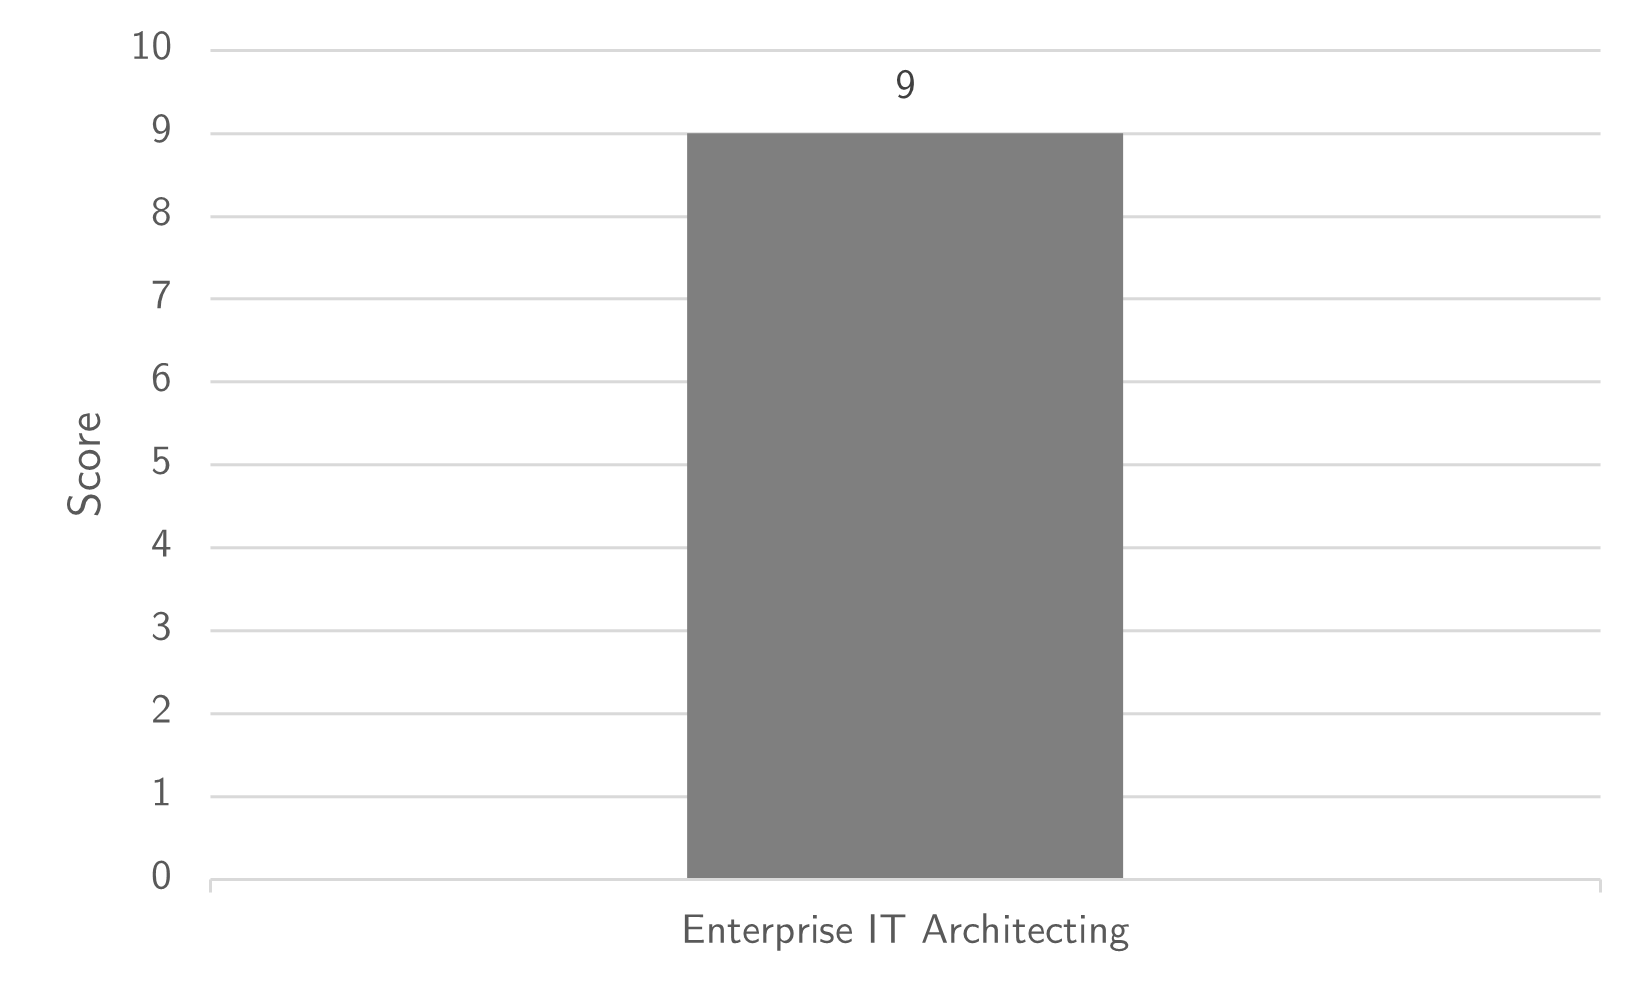
\includegraphics[width=\textwidth]{images/qdaeaschool}
		\caption{QDA EA school of thought}
		\label{fig:qdaea}
	\end{subfigure}
	\caption{Results of QDA Learning organisation and EA school of thought}
	\label{fig:resultsofqda}
\end{figure}

\subsection{Results of QDA of new possible attributes}
\label{sub:resultsqdanewaatributes}
\begin{figure}[H]
	\centering
	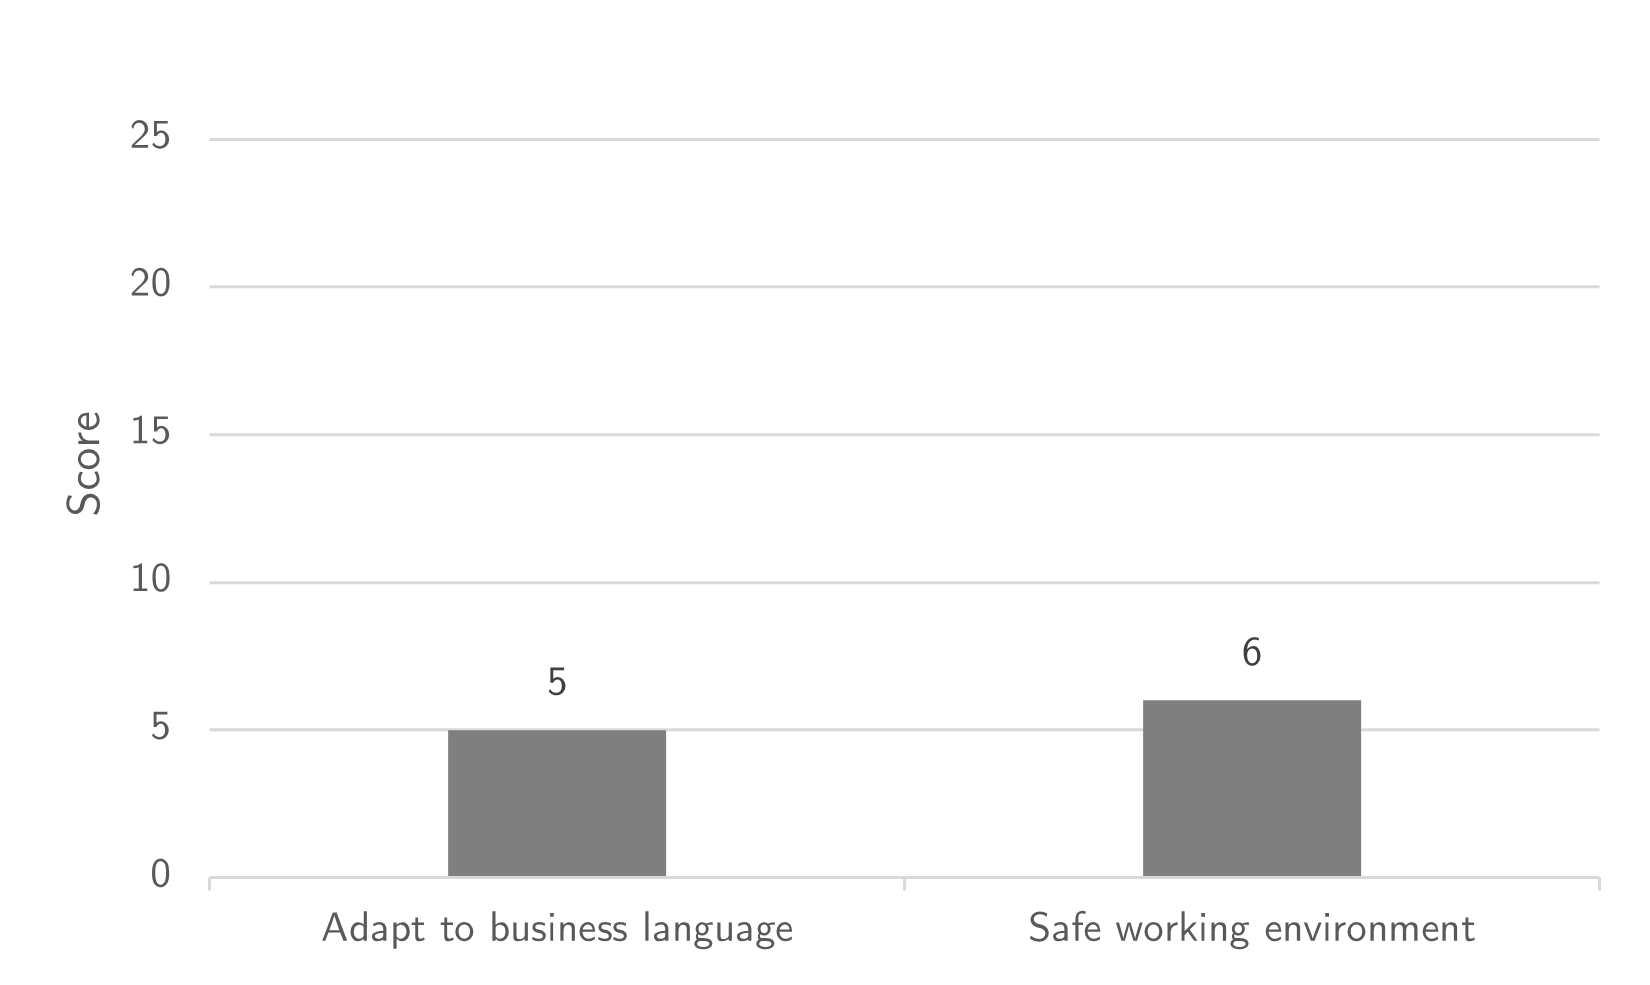
\includegraphics[width=0.475\textwidth]{images/qdanewfindings}
	\caption[QDA new attributes]{QDA new attributes}
	\label{fig:qdanewfindings}
\end{figure}


\subsection{Identified attributes as possible success factors}
\label{sub:identifiedattributesaspossiblesf}
\begin{table}[H]
	\begin{center}
		%\resizebox{\textwidth}{!}{%
			\begin{tabular}{@{}ll@{}}
				\toprule%
				\textbf{Attribute} & \textbf{Category}  \\%
				\midrule%
				\Gls{optionality} & \Gls{amplifyvariety} \\%
				\Gls{nonmonotonicity} & \Gls{amplifyvariety} \\%
				\Gls{selforganisation} & \Gls{amplifyvariety} \\%
				\Gls{failfast} & \Gls{amplifyvariety} \\%
				\Gls{resourcestoinvest} & \Gls{amplifyvariety} \\%
				\Gls{senecabarbell} & \Gls{amplifyvariety} \\%
				\Gls{systeminenvironment} & \acrshort{ea} \Gls{enterpriseecologicaladaptation} \\%
				\Gls{holisticsystemicstance} & \acrshort{ea} \Gls{enterpriseecologicaladaptation} \\%
				\Gls{organisationallearning} & \acrshort{ea} \Gls{enterpriseecologicaladaptation} \\%
				\Gls{environmentallearning} & \acrshort{ea} \Gls{enterpriseecologicaladaptation} \\%
				\Gls{intraorganisationalcoherency} & \acrshort{ea} \Gls{enterpriseecologicaladaptation} \\%
				\Gls{systeminenvironmentcoevolutionlearning} & \acrshort{ea} \Gls{enterpriseecologicaladaptation} \\%
				\Gls{safeworkingenvironment} & New finding \\%
				\Gls{adapttobusinesslanguage} & New finding \\%
				\bottomrule%
			\end{tabular}
		%}
		\caption{Possible success factors identified from interviews}
	\end{center}
\end{table}